\documentclass[12pt,letterpaper]{exam}
\usepackage[lmargin=1in,rmargin=1in,tmargin=1in,bmargin=1in]{geometry}
\usepackage{../style/exams}

% -------------------
% Course & Exam Information
% -------------------
\newcommand{\course}{MAT 308: Exam 1}
\renewcommand{\term}{Fall -- 2023}
\newcommand{\examdate}{10/12/2023}
\newcommand{\timelimit}{`$\infty$' Minutes}

\setbool{hideans}{true} % Student: True; Instructor: False

% Logical Circuits
\usepackage{circuitikz}
\usetikzlibrary{shapes.gates.logic.US,shapes.gates.logic.IEC}

\newcommand{\blank}[1]{\underline{\hspace{#1}}} % Blank Underline


% -------------------
% Content
% -------------------
\begin{document}

\examtitle
\instructions{Write your name on the appropriate line on the exam cover sheet. This exam contains \numpages\ pages (including this cover page) and \numquestions\ questions. Check that you have every page of the exam. Answer the questions in the spaces provided on the question sheets. Be sure to answer every part of each question and show all your work. If you run out of room for an answer, continue on the back of the page --- being sure to indicate the problem number.} 
\scores
\bottomline
\newpage

% ---------
% Questions
% ---------
\begin{questions}

% Question 1
\newpage
\question[10] Consider the logical expressions $\neg (P \wedge Q)$ and $(P \to \neg Q) \vee (\neg P \wedge \neg Q)$.
	\begin{enumerate}[(a)]
	\item Show that these two expressions are logically equivalent by constructing the truth table for both expressions. 
	\item Show that $\neg (P \wedge Q) \equiv (P \to \neg Q) \vee (\neg P \wedge \neg Q)$ by `simplifying' the expression $(P \to \neg Q) \vee (\neg P \wedge \neg Q)$. 
	\item Without computing the truth table for $P \wedge Q \Leftrightarrow (P \to \neg Q) \vee (\neg P \wedge \neg Q)$, determine whether this expression is a tautology, contradiction, or neither. Explain how you came to your conclusion. 
	\end{enumerate}



% Question 2
\newpage
\question[10] Consider the digital logic circuit given below. We shall find a simpler circuit that has the same `behavior', i.e. input-output table, as the given circuit. 
	\[
	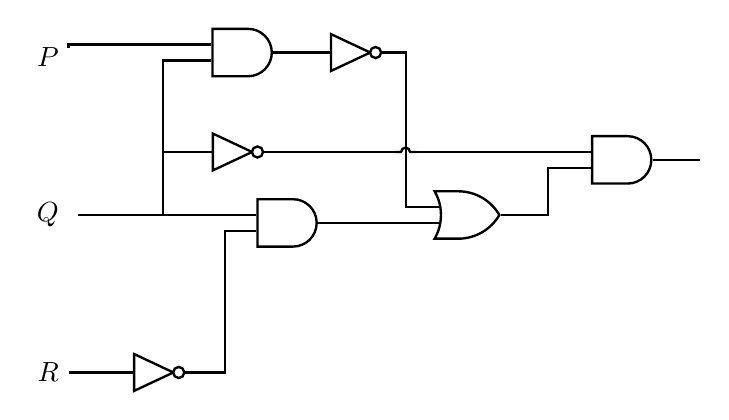
\begin{tikzpicture}
	\node (p) at (0,4) {}; \node[left] at (p) {$P$}; % P
	\node (q) at (0,2) {}; \node[left] at (q) {$Q$}; % Q
	\node (r) at (0,0) {}; \node[left] at (r) {$R$}; % R
	
	\node[not gate US, draw, line width= 0.03cm] at (1,0) (not1) {}; % lower NOT
	\node[and gate US, draw, line width= 0.03cm] at (2.75,1.8997) (and1) {}; % middle AND
	\node[not gate US, draw, line width= 0.03cm] at (2,2.8) (not2) {}; % middle NOT
	\node[and gate US, draw, line width= 0.03cm] at (2.18,4.063) (and2) {}; % upper AND
	\node[not gate US, draw, line width= 0.03cm] at (3.5,4.063) (not3) {}; % upper NOT
	\node[or gate US, draw, line width= 0.03cm] at (5,2) (or1) {}; % OR
	\node[and gate US, draw, line width= 0.03cm] at (7,2.69997) (and3) {}; % right AND
	
	\draw[line width= 0.03cm] (r) |- (not1.input); % r to lower NOT
	\draw[line width= 0.03cm] (q) -- (1.2,2) |- (and1.input 1); % q to middle AND
	\draw[line width= 0.03cm] (not1) -- ([xshift=0.5cm]not1.output) |- (and1.input 2); % lower NOT to AND
	\draw[line width= 0.03cm] (1.2,2) |- (not2.input); % q to middle NOT
	\draw[line width= 0.03cm] (p) |- (and2.input 1); % p to upper AND
	\draw[line width= 0.03cm] (1.2,2) |- (and2.input 2); % q to upper AND
	\draw[line width= 0.03cm] (and2.output) |- (not3.input); % upper AND to upper NOT
	\draw[line width= 0.03cm] (and1.output) -- ([xshift=0.6cm]and1.output) |- (or1.input 2); % middle AND to OR
	\draw[line width= 0.03cm] (not3.output) -- ([xshift=0.3cm]not3.output) |- (or1.input 1); % upper NOT to OR
	\draw[line width= 0.03cm] (or1.output) -- ([xshift=0.6cm]or1.output) |- (and3.input 2); % OR to right AND
	\draw[line width= 0.03cm] (not2.output) -- (4.16,2.8) to[crossing] (4.4,2.8) |- (and3.input 1); % middle NOT to right AND
	\draw[line width= 0.03cm] (and3.output) -- ([xshift=0.6cm]and3.output); % output wire
	\end{tikzpicture}
	\]

\begin{enumerate}[(a)]
\item Find the logic expression corresponding to this circuit. 
\item Simplify the logical expression in (a) as much as possible.
\item Construct the digital logic circuit corresponding to your answer in (b).
\end{enumerate}



% Question 3
\newpage
\question[10] Let $z, q$ be free variables with universe $\mathbb{Z}$ and $\mathbb{Q}$, respectfully. Define the predicate $P(z, q) \colon z \neq 0 \to qz= 1$. Consider the quantified statement\dots
	\[
	(\forall z)(\exists q) P(z, q)
	\]

\begin{enumerate}[(a)]
\item Write the quantified statement above as a complete English sentence. 
\item Determine whether the given quantified statement is true or false. Be sure to justify your answer. 
\item Write the negation, converse, and contrapositive of the given quantified statement as complete English sentences. 
\end{enumerate}



% Question 4
\newpage
\question[10] Define sets $A, B, C, D$ as given below with universe $\mathcal{U}= (-\infty, \infty)$. 
	\[
	\begin{aligned}
	A&= (-10, 10) \qquad& C&= [5, 20) \\[0.1cm]
	B&= (-15, 0] & D&= [-6, 6]
	\end{aligned}
	\]

\begin{enumerate}[(a)]
\item $B^c$
\item $A \Delta C$
\item $D \setminus B$
\item $(A \cup B)^c$
\item $A \cap (B \cup C)$
\end{enumerate}



% Question 5
\newpage
\question[10] Let $X= \{ a, b, c \}$ and $Y= \{ 1, 2 \}$. 
	\begin{enumerate}[(a)]
	\item Compute $\mathcal{P}(X)$.
	\item Compute $\mathcal{P}(X) \times Y$. 
	\item Compute $|\mathcal{P}(X) \times Y|$.
	\item Is $\big( \{ b, a, a \}, 1 \big) \in \mathcal{P}(X) \times Y$?
	\end{enumerate}



% Question 6
\newpage
\question[10] For natural numbers $n$, let $A_n= \left[ -\frac{1}{n}, \frac{n + 1}{n} \right)$, and for real numbers $x$, let $B_x= (x - 1, x + 1)$. Compute the following:
	\begin{enumerate}[(a)]
	\item $\displaystyle \bigcup_{n \in \mathbb{N}} A_n$
	\item $\displaystyle \bigcap_{n \in \mathbb{N}} A_n$
	\item $\displaystyle \bigcup_{x \in \mathbb{R}} B_x$
	\item $\displaystyle \bigcap_{x \in \mathbb{R}} B_x$
	\end{enumerate}



% Question 7
\newpage
\question[10] Let $\Phi \colon \mathbb{R} \to \mathbb{R}$ be given by $x \mapsto 2x^2 + 11x - 6$. 
	\begin{enumerate}[(a)]
	\item Is $7 \in \im \Phi$? Explain. 
	\item Is $-11 \in \Phi^{-1}(-5)$? Explain. 
	\item Compute $\im \Phi$.
	\item Compute $\Phi^{-1}(0)$. 
	\item Is $(3, 11)$ on the graph of $\Phi$? Explain. 
	\item Is $\Phi$ a decreasing function? Explain.  
	\item Is $\Phi$ a negative function? Explain. 
	\end{enumerate}

\newpage 
\begin{center} {\itshape --- Continued Space for Problem~7 ---} \end{center}
\newpage

	

% Question 8
\newpage
\question[10] Complete the following parts, being sure to fully justify your reasoning:
	\begin{enumerate}[(a)]
	\item Is the function $f: \mathbb{R}^2 \to \mathbb{R}$ given by $f(x, y)= x^2 + y^3 - 7$ injective?
	\item Is the function $g: \mathbb{R} \to (-\infty, 10]$ given by $x \mapsto 10 - (x - 3)^2$ surjective?
	\item Is the function $h: \mathbb{R} \to \mathbb{R}$ given by $h(x)= \pi x - \sqrt{2}$ bijective? 
	\end{enumerate}



% Question 9
\newpage
\question[10] Below is a partial proof of the fact that if $A, B, C$ are sets, then $A \times (B \setminus C)= (A \times B) - (A \times C)$. By filling in the missing portions, complete the partial proof below so that it is a correct, logically sound proof with `no gaps.' \pspace

{\textbf Proposition.} If $A, B, C$ are sets, then $A \times (B \setminus C)= (A \times B) - (A \times C)$. \pspace

{\itshape Proof.} To show that $A \times (B \setminus C)= (A \times B) - (A \times C)$, we need to show that $A \times (B \setminus C) \subseteq (A \times B) - (A \times C)$ and $(A \times B) - (A \times C) \subseteq A \times (B \setminus C)$. \par\vspace{2\baselineskip}

If $A \times (B \setminus C)= \varnothing$, we clearly have $A \times (B \setminus C) \subseteq (A \times B) - (A \times C)$. Similarly, if $(A \times B) - (A \times C)= \varnothing$, then we have $(A \times B) - (A \times C) \subseteq A \times (B \setminus C)$. Now assume that $A \times (B \setminus C)$ and $(A \times B) - (A \times C)$ are nonempty. \par\vspace{2\baselineskip}

$A \times (B \setminus C) \subseteq (A \times B) - (A \times C)$: Let $(x, y) \in A \times (B \setminus C)$. We want to show that \pspace $(x, y) \in (A \times B) - (A \times C)$. By definition, $(x, y) \in A \times (B \setminus C)$ implies that \blank{3cm} \pspace and \blank{3cm}. Because $y \in B \setminus C$, we know that \blank{4cm} and \pspace \blank{4cm}. Now $x \in A$ and $y \in B$, so that $(x, y) \in A \times B$. Because $y \notin C$, \pspace we know that $(x, y) \notin A \times C$. Because \blank{4cm} and \blank{4cm}, \pspace we know that $(x, y) \in (A \times B) - (A \times C)$. But then if $(x, y) \in A \times (B \setminus C)$, we know \pspace that $(x, y) \in (A \times B) - (A \times C)$. Therefore, \blank{6cm}. \par\vspace{2\baselineskip}

$(A \times B) - (A \times C) \subseteq A \times (B \setminus C)$: Let \blank{6cm}. We want to \pspace show that $(x, y) \in A \times (B \setminus C)$. Because $(x, y) \in (A \times B) - (A \times C)$, we know that \pspace \blank{4.5cm} and \blank{4.5cm}. By definition, because $(x, y) \in$ \pspace $A \times B$, $x \in A$ and $y \in B$. We also know that $(x, y) \notin A \times C$. So either \blank{4cm} \pspace or \blank{4cm}. But we know that $x \in A$, so that it must be that $y \notin C$. But \newpage

\phantom{.}\par\vspace{0.3cm} then $y \in B$ and \blank{3cm}, which implies that $y \in B \setminus C$. Because \blank{3cm} \pspace and $y \in B \setminus C$, we know that $(x, y) \in A \times (B \setminus C)$. Then if $(x, y) \in (A \times B) - (A \times C)$, \pspace we know \blank{6cm}. Therefore, $(A \times B) - (A \times C) \subseteq A \times (B \setminus C)$. \par\vspace{2\baselineskip}

Because \blank{5.5cm} and \blank{5.5cm}, we know \pspace that $A \times (B \setminus C)= (A \times B) - (A \times C)$. \qed



% Question 10
\newpage
\question[10]  Below is a partial proof of results about the surjectivity of functions. By filling in the missing portions, complete the partial proof below so that it is a correct, logically sound proof with `no gaps.' \pspace

{\textbf Proposition.} Let $A, B, C$ be sets and $f: A \to B, g: B \to C$ be functions. 
	\begin{enumerate}[(i)]
	\item If $f, g$ are surjective, then $g \circ f$ is surjective. 
	\item If $g \circ f$ is surjective, then $g$ is surjective. 
	\end{enumerate} \pspace

{\itshape Proof.} 

\begin{enumerate}[(i)]
\item Suppose that $f, g$ are surjective. We want to show that \blank{5cm}. \pspace We need to show that if \blank{3cm}, there exists \blank{3cm} such that \pspace $(g \circ f)(a)= c$. Because $g$ is surjective, there exists $b \in B$ such that \blank{3cm}. \pspace Because \blank{4.5cm}, there exists $a \in A$ such that $f(a)= b$. But then \pspace \blank{7cm}. Therefore, $g \circ f$ is surjective. \par\vspace{2\baselineskip}

\item Assume that \blank{5.5cm}. We want to show that $g$ is surjective. \pspace We need to show that if \blank{3cm}, there exists \blank{3cm} such that \pspace \blank{4cm}. Let $c \in C$. Because $g \circ f: A \to C$ is surjective, there exists \pspace $a \in A$ such that $(g \circ f)(a)= c$. We know that $(g \circ f)(a)= g\big( f(a) \big)$. Because \pspace $f: A \to B$, we know that $f(a) \in $ \blank{3cm}. Then there is \blank{3cm} \pspace such that $b= f(a)$. Then $g(b)= $ \blank{4cm}. Therefore, $g$ is surjective. 
\end{enumerate} \qed


\end{questions}
\end{document}